\documentclass[10pt, french, a4paper]{article}

\usepackage[authoryear]{natbib}


\usepackage[textwidth=14cm]{geometry}
\usepackage{babel}
\usepackage{graphicx}
\usepackage{hyperref}	
\usepackage{enumitem}
\usepackage{tabularx}
\usepackage{amsmath}

\title{Mémoire : L’éthique des intelligences artificielles et le contrôle de leurs impacts sociaux}
\author{Nathan Lauga}
\date{\today}

\begin{document}

\maketitle

\newpage
\tableofcontents

\newpage
\begin{abstract}

    Ceci est l'avant-propos.

\end{abstract}

% ====== INTRODUCTION ====== %

\newpage
\section{Introduction}


Aujourd'hui, les intelligences artificielles omniprésentes
Prennent des décisions sans que nous nous en aperçevions (pub, YT)
Perf impressionnantes : (2017 jeu de go, AlphaGo et 2 semaines MIT, antibiotique)
et facilité de création ==> + en + d'IA
Conséquence : des IA qui font parlé dans les médias car biaisée (ex Amazon)
La question de pouvoir anticiper les biais et la transparence des IA est fondamentale et d'actualité ==> mon mémoire

\paragraph{Problématique}
Dans un contexte où les intelligences artificielles sont omniprésentes et que les données deviennent le nouveau pétrole, 
comment déterminer si une IA est éthique et par conséquent limiter les impacts sociaux sous-jacents ?


% ====== IA ET ETHIQUE ====== %

\newpage
\section{L'IA et l'éthique une association forcée}

% ------ IA ------ %

\paragraph{Définition des termes}
\begin{itemize}
    \item \textbf{Algorithme} : Il s'agit d'une suite d'instruction permettant de résoudre un problème donné. Une IA correspond à un algorithme plus ou moins complexe.
    \item \textbf{Modèle} : C'est une descritption mathématique qui se génère à partir d'observation, où plus précisément dans le domaine de l'intelligence artificielle à partir des données. Il sera souvent utilisé en tant que synonyme d'IA. 
    \item \textbf{Singularité} : Ce terme décrit le moment où une intelligence artificielle aura atteint les capacités intellectuelles de
    l’Homme. Cela peut être également assimiler au jour où l'homme n'aura plus la capacité de rivalisé avec les machines.
    \item \textbf{Biais} : fait référence à une déviation de la réalité, un moyen de contourner. Très souvent associé aux biais cognitifs chez l'espèce humaine.
\end{itemize}

\subsection{L'intelligence artificielle, quand les machines révolutionnent le monde}
\label{subsec:ia}

\paragraph{}
L’intelligence artificielle, un mot qui, depuis quelques années, semble être sur toutes les bouches. Bien que l’imaginaire collectif puisse entrevoir des machines humanoïdes capable de détruire l’homme (e.g. Terminator\footnote{Le film "Terminator", réalisé par James Cameron et sortie en 1985, représente un cyborg du futur envoyé par des robots, qui a pour mission de tuer Sarah Connor, mère du chef des résistants humains.}), les technologies actuelles ne nous offrent pas encore un spectacle digne d’Hollywood. Évidemment, le terme en lui-même donne une illusion humaine puisque le mot "intelligence" est présent. Il faut tout de suite dissocier cette intelligence dite "artificielle" de celle qui est associée aux hommes, l’intelligence dite "naturelle".

\paragraph{}
En informatique, la recherche sur l’intelligence artificielle est définie comme l’étude des "agents intelligents", soit n’importe quel appareil qui perçoit son environnement et prend des décisions qui maximisent ses chances d’atteindre son objectif \citep{poole_computational_1997}. Un exemple illustre cette définition : dans les jeux d’échecs, un agent intelligent pourra, en connaissant les règles du jeu, effectuer des coups et son objectif, qu’il cherchera à atteindre, sera de battre son adversaire.

\subsubsection{Un commencement agité}

\paragraph{}
Le terme qui aujourd’hui, est très évocateur, a été utilisé pour la première fois en 1956 par John McCarthy, lors de la conférence de Darthmouth, conférence qui est considérée comme l’acte de naissance de l’intelligence artificielle en tant que domaine de recherche autonome \citep{solomonoff_time_1985}. Bien sûr, cette notion bien que sans nom précis jusqu’à cette conférence, n’était pas inexistante.

\paragraph{}
L’apparition de technologies impressionnantes a été prédite juste avant que les bombes atomiques ne tombent sur le Japon \citep{bush_as_1945}. Parmi celles-ci, il est possible de trouver les ordinateurs, Internet, la reconnaissance vocale et d’autres concepts révolutionnaires, qui peuvent être définit comme des systèmes qui pourrait amplifier le savoir et la connaissance de chacun. Les technologies modernes confirment bel et bien cette hypothèse.

\paragraph{}
Une idée de machines intelligentes se propage ensuite notamment au travers du terme cybernétique en tant que théorie entière de la commande et de la communication, aussi bien chez l’animal que dans la machine \citep{wiener_cybernetics;_1961}.

\paragraph{}
Le concept d’une technologie, qui pourrait servir l’homme jusqu’à asservir ses besoins intellectuels, est donc apparue, mais cela reste un peu vague et ne ressemble pas à une notion de machine intelligente au même niveau que l’homme. C’est cinq ans plus tard, en 1950, qu’Alan Turing\footnote{Alan Turing, étant également considéré comme le père de l’informatique, a notamment donné son nom au "Prix Turing", récompensant une personne chaque année, pour sa contribution au monde de l’informatique.}, considéré comme le père de l’intelligence artificielle, publie un article qui révolutionna le monde de l’informatique \citep{turing_i.computing_1950}.

\paragraph{}
En résumé, il a soulevé la question désormais célèbre "Can machine think ?"\footnote{Traduction : Les machines peuvent-elles penser ?} . Cette interrogation est très contradictoire, surtout en 1950, puisque le terme "machine" et "penser", ne peuvent être définis d’une façon qui puisse satisfaire tout le monde. Afin de résoudre le conflit de cette contradiction, Turing a proposé une solution, élégante, étant le fameux "Test de Turing".

\paragraph{}
Le Test de Turing, est construit de la façon suivante : si une machine peut tenir une discussion avec un humain (au travers d’une messagerie par exemple), sans que la femme ou l’homme ne puisse distinguer qu’il s’agisse d’un humain ou d’une machine alors la définition du test dira que cette machine est "pensante". Il s’agit d’une proposition très importante dans la philosophie de l’intelligence artificielle \citep{pinar_saygin_turing_2000}.

\paragraph{}
Au travers de la notion révolutionnaire d'une machine dite "pensante", un engouement est naturellement apparu autour des machines, des déclarations chocs sont faites comme "d’ici dix ans un ordinateur sera le champion du monde des échecs" \citep{simon_heuristic_1958} ou encore "des machines seront capables, d’ici vingt ans, de faire tout travail que l’homme peut faire" \citep{simon_shape_1965}. Il n’est pas le seul à faire de telles affirmations et celles-ci mènent à une attente très élevée concernant les possibilités des algorithmes intelligents, mais comme souvent lorsque les attentes sont élevées une phase de déception s’ensuit.

\paragraph{}
Bienvenue dans le premier hiver de l’histoire de l’intelligence artificielle. Comme une bulle qui aurait éclaté, la recherche a ralenti d’un coup, ainsi que le budget consacré au domaine. Les causes en sont multiples. Il est possible de retrouver entre autres, la limite de la puissance de calcul des ordinateurs ou encore le manque de base de connaissances du monde par les ordinateurs (manque de données). En effet, les travaux, qui portaient sur le langage naturel, ne pouvaient pas être extrêmement poussés puisque le stockage de la mémoire la limitait à vingt mots \citep{crevier_ai:_1992}.

\paragraph{}
Pour beaucoup ce secteur a été enterré, mais arrivèrent les systèmes experts, programmes qui allient algorithme et connaissance métier. Ce concept qui comme le Soleil au printemps fit fondre la neige du premier hiver.

\paragraph{}
L’histoire se répéta malheureusement dans les années 90 : trop d’attente pour une réalité en dessous de l’imaginaire. Conséquence, une nouvelle période froide dans ce domaine et un désenchantement populaire.

\begin{center}
    \begin{figure}[hbt!]
        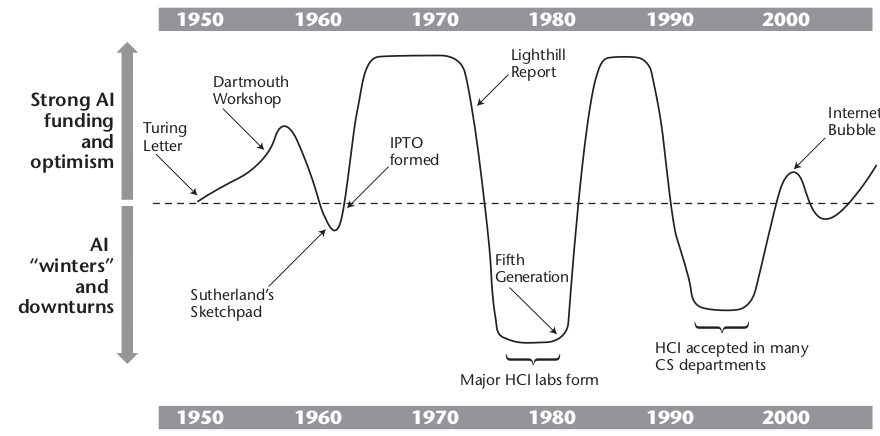
\includegraphics[width=\textwidth]{images/grudin_2009_changing_seasons_ai.png}
        \caption{Les saisons changeantes de l'IA \citep{grudin_ai_2009}}
    \end{figure}
\end{center}

\paragraph{}
Ci-dessus un résumé des débuts de l’histoire de l’intelligence artificielle avec en abscisse les années et en ordonnées l’attente autour de ce secteur. Sur le graphique, certains évènements majeurs de l’histoire du domaine en question.

\subsubsection{La machine plus forte que l'homme ?}

\paragraph{}
Le froid qui s’était abattu sur l’intelligence artificielle peut laisser supposer que les pensées révolutionnaires n’auraient pu se réaliser, mais la machine, sans oublier les développeurs, ont plus d’un tour dans leur sac. Dans les années 1990, IBM sortit une machine nommée "Deep Blue". Elle a été construite dans le but de jouer aux échecs et surtout de battre le meilleur joueur d’échec du monde. Après un échec en 96, la surprise fut totale quand en 1997, le vainqueur ne put lever les bras pusiqu’il s’agissait de Deep Blue \citep{krauthammer_be_1997}. L’imaginaire d’une machine plus intelligente que l’homme refit surface dans certains esprits.

\paragraph{}
Malgré cet exploit, la force de cet algorithme était "juste" de pouvoir calculer très rapidement en parallélisant les calculs et donc d’anticiper les coups de son adversaire plus facilement que le cerveau humain \citep{hsu_deep_1995}. Il est possible de comparer cela à une calculatrice appliquant une multiplication complexe et affichant la réponse en un claquement de doigts, alors que pour un homme cela est une tout autre histoire.

\paragraph{}
La révolution qui a mené l’intelligence artificielle à sa place aujourd’hui n’est pas uniquement due à une grande bête de calcul, la raison principale est le "machine learning" ou en français l’apprentissage de la machine.

\paragraph{}
Un bébé regardera ses parents, sa famille et son entourage pour apprendre à marcher, un algorithme de "Machine Learning", lui n’a pas d’œil pour regarder ,mais du code pour analyser les données fournies par les développeurs. Un sortilège utilisant pour baguette magique, des formules mathématiques et statistiques permettant alors de généraliser à partir de ce que l’intelligence artificielle a en base d’apprentissage.

\paragraph{}
Cette catégorie d’intelligence artificielle est aujourd’hui la grande dominante du marché. Elle se découpe en différentes catégories, l’une des plus utilisées est l’apprentissage supervisé consistant à donner à la machine des données dites "labellisées", soit qui possèdent déjà la réponse à la problématique (e.g. prédire la météo en utilisant les données des années précédentes en indiquant en label le temps qu’il faisait réellement). Ensuite, l’apprentissage non supervisé, lui se distinguera puisqu’il n’y aura pas de label identifié, l’objectif est de trouver des patterns, de segmenter ou de détecter des anomalies.

\paragraph{}
Au travers de ces deux catégories, une vaste quantité d’algorithmes existent, de la simple régression linéaire, en passant par le traditionnel arbre de décision, la catégorie d’algorithme ayant permis de faire un grand pas, sans discussion possible, est celle des réseaux de neurones.

\paragraph{}
Un mot assez frappant, puisqu’il associe directement des machines à l’homme, plus précisément au cerveau humain. Or, non en dehors de la forme, ces réseaux de neurones ne sont pas du tout le cerveau humain. La logique est similaire : des "neurones" prenant des informations en entrée pour en ressortir une autre information à son tour vers un niveau suivant. Bien que cela puisse raviver l’illusion d’une machine aussi intelligente que l’homme, les algorithmes actuels peuvent être décrits comme intelligences artificielles "stupides" car elles n’appliquent, que ce pour quoi elles ont été créées, avec des niveaux de performances parfois, bluffant. La déclaration d’Andrew Moore \citep{newsflash_ai_2018}, responsable de Google Cloud AI, le confirme "AI is currently, very, very stupid"\footnote{Traduction : l’IA est actuellement, très, très stupide.}.

\paragraph{}
L’un des portraits qui peut le mieux décrire la force de frappe de cette génération d’IA, peut être associée à l’histoire de la défaite d’un homme au jeu de Go. Le jeu de Go est l’un des jeux considérés comme les plus complexes au monde, soit un jeu qui pour l’homme devait lui rester en main pour de longues décennies après la montée des IA pour les échecs.


\begin{figure}[hbt!]
    \centering
    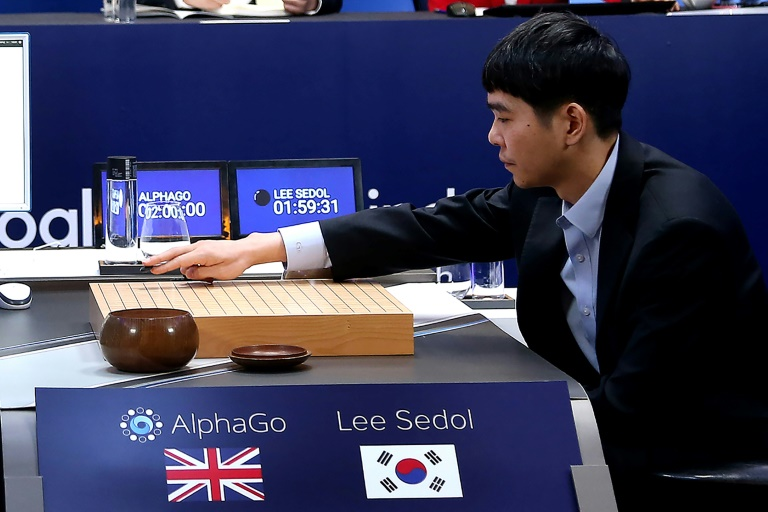
\includegraphics[width=0.8\textwidth]{images/alphago_lee_sedol.jpg}
    \caption{Lee Se-dol, champion de Jeu de Go jouant un coup face à AlphaGo \citep{noauthor_alphago_2017}}
    \label{fig:proba_super_ia}
\end{figure}

\paragraph{}
Une entreprise spécialisée dans la création d’algorithmes intelligents, DeepMind, s’est lancée dans ce défi au cours de la décennie actuelle. Son premier "enfant", baptisé "AlphaGo", s’entraîna sur des parties jouées par des joueurs professionnels de Go. En 2016, elle se présenta en Corée du Sud dans le but d’affronter le champion du monde Lee Se-dol en cinq parties. La fin de l’histoire fit un bis repetita avec Deep Blue et AlphaGo triompha de l’humain \citep{deepmind_alphago_2016}.

\paragraph{}
Cette victoire fit des titres sensationnels dans les médias, mais le plus spectaculaire n’est pas cette victoire. Un peu plus d’un an plus tard, DeepMind accoucha de la sœur (ou frère, le genre n’a que peu d’importance) cadette d’AlphaGo : AlphaGoZero. Le nom n’est pas anodin au vu de l’apprentissage de cette machine. Contrairement à l’algorithme "champion du monde", la logique n’est pas de se baser sur des matchs existants, mais de lui apprendre les règles du jeu, puis de laisser l’algorithme s’affronter tout seul pendant un certain temps, jusqu’à par lui-même redécouvrir les coups des débutants, les stratégies que les humains ont mis un millénaire à apprendre pour enfin complètement dépasser ces méthodes presque moyenâgeuses \citep{silver_mastering_2017}. Pour l’anecdote AlphaGoZero fut triomphant d’AlphaGo sur un score de cent matchs à zéro.

\paragraph{}
Cet algorithme basé sur une méthode d’apprentissage non supervisé a continué d’être utilisé par DeepMind et d’autres entreprises pour aller jusqu’à, récemment, battre des joueurs professionnels de "StarCraft II", un jeu vidéo \citep{vinyals_alphastar:_2019}.

\paragraph{}
Ce récit, qui dicte des exploits qualifiables de surhumains, n’est qu’un exemple sensationnel et qui a eu de la popularité en dehors de la communauté centrée autour des algorithmes intelligents. Créer des musiques \citep{medeot_structurenet:_2018}, créer des peintures au format numérique \citep{mordvintsev_inceptionism:_2015}, reproduire des visages humains \citep{karras_style-based_2018}, imiter un discours d’un président américain \citep{suwajanakorn_synthesizing_2017}, ces tâches ont bel et bien été accomplies par des intelligences artificielles.

\paragraph{}
Tout ceci a fait resurgir un sentiment similaire aux périodes précédents les deux dernières périodes hivernales que l’IA a connu, un sentiment de machines bien plus performantes que l’homme, pouvant être même plus intelligentes que l’être humain. Or, comme évoqué précédemment, elles ne réalisent que ce pourquoi elles ont été créées. De plus, aucune n’a réussi à passer le test de Turing, qui semble être la mesure qui permettra de déterminer leur intellect "équivalent" au nôtre. Cette période, appelée singularité\footnote{Ce terme décrit le moment où une intelligence artificielle aura atteint les capacités intellectuelles de l’Homme.}, est-elle pour bientôt ?

\paragraph{}
Penser qu’une machine aussi intelligente que l’homme est pour très bientôt ou très longtemps, est digne d’un fantasme dans l’imaginaire collectif. Il ne s’agit pas là forcément de la meilleure opinion afin d’avoir la meilleure prédiction à la question du passage de la singularité. Des chercheurs d’Oxford et de Yale ont décidé d’interroger un grand nombre de chercheurs du domaine de l’intelligence artificielle du monde entier afin de déterminer une approximation sur la singularité \citep{grace_when_2017}. Les résultats sont très variés, mais une courbe a émergé de leur sondage (voir figure \ref{fig:proba_super_ia}).

\begin{figure}[hbt!]
    \centering
    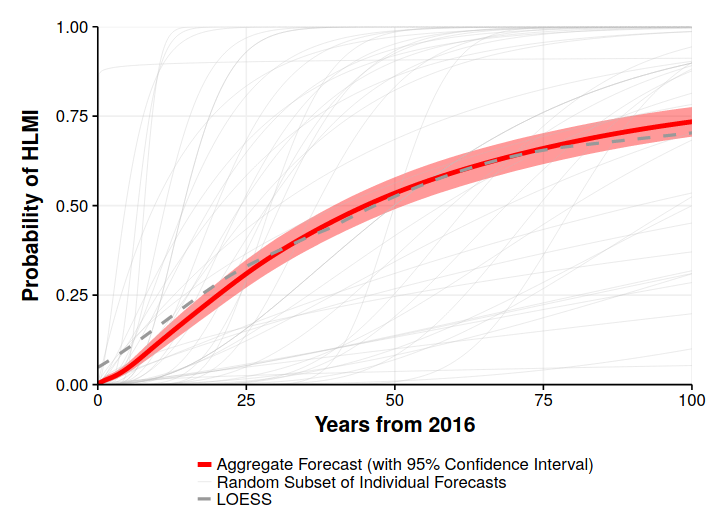
\includegraphics[width=0.9\textwidth]{images/grace_2017_proba_super_ia.png}
    \caption{Probabilité d'une super-intelligence à partir de 2016 \citep{grace_when_2017}}
    \label{fig:proba_super_ia}
\end{figure}

\paragraph{}
Ce graphique détaille la probabilité d’une "HLMI" soit "High-level machine intelligence" synonyme de la singularité à partir de l’année 2016. Les traits gris dans le fond correspondent à des réponses individuelles et il est remarquable de voir leur écart. L’information à retenir sur ce graphique est donc la ligne rouge indiquant une prévision agrégée qui nous indique une probabilité dépassant les cinquante pourcents d’ici cinquante ans.

\paragraph{}
De plus, cette même recherche a posé des questions plus diverses comme notamment la possibilité qu’un humain soit battu au jeu de Go et la réponse moyenne était que cette tâche serait réalisée d’ici 2028, pourtant moins d’un an après la publication de cette recherche AlphaGo a triomphé. Sur la figure suivante, il est possible d’observer que les questions sont posées sur le remplacement de femmes et hommes et les deux questions en haut poussent la réflexion jusqu’à une IA pouvant rechercher pour améliorer les algorithmes intelligents créant un parallèle avec l’humain et la médecine. Puis en dernier, la question posée s’axe sur l’automatisation totale du travail humain par les intelligences artificielles.

\begin{figure}[hbt!]
    \centering
    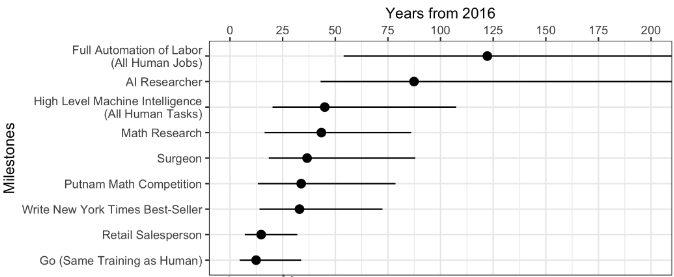
\includegraphics[width=0.9\textwidth]{images/grace_2017_chrono_estim_ia.png}
    \caption{Chronologie des estimations qu’une IA achève des tâches humaines \citep{grace_when_2017}}
    \label{fig:chrono_estim_ia}
\end{figure}

\paragraph{}
Pousser la réflexion à la question de ce que sera le monde dans plusieurs décennies est déjà suffisamment complexe sur des questions pouvant être plus fondamentales (écologie, collapsologie, social, consommation, etc.). Cela n’empêche pas d’y réfléchir : les IA seront-elles nos sauveuses ? Notre talon d’Achille ? Ou bien vivront-elles une vie à nos côtés sans changer nos habitudes ? Entre pessimisme et utopie, chacun peut se faire son avis, rien n’est encore écrit. Même si les questions sont soulevées, pour pouvoir se faire sa propre idée, assimiler ce qu'est une intelligence artificielle de nos jours est fondamental.

\subsubsection{Derrière la notion d'IA aujourd’hui}
\label{subsubsection:ia_auj}

\paragraph{}
La constatation des progrès des intelligences artificielles ne laisse pas indifférent pour sûr, par conséquent bien assimiler leur utilité de nos jours permet une meilleure compréhension du monde moderne. Quand il est discuté d'IA, de nos jours, ce qui est presque tout le temps utilisé correspond à du Machine Learning.

\paragraph{}
Le Machine Learning ou l'apprentissage de la machine est une discipline d'étude de l'intelligence artificielle. Elle se fonde sur des approches mathématiques et statistiques permettant d'apprendre à partir des données fournies. De plus, il est possible de la retrouver presque partout dans notre quotidien : dans les téléphones, les montres connectées ou encore les véhicules.

\paragraph{}
Le rayonnement de ce domaine est tellement fort que dans notre société capitaliste qui carbure à l'argent, plus de 9,8 milliards de dollars ont été investis en 2018. Cette somme représente une augmentation d'environ 72\% par rapport à 2018 \citep{columbus_25_2019}.

\paragraph{}
La logique d'apprentissage par l'exemple de cette discipline peut être comprise par l'analogie d'un enfant en bas âge qui veut apprendre à marcher. Au début, il voit ses parents marcher et enregistre comment son corps pourrait s'approprier le mouvement. Puis, il essaye de le reproduire, au début il tombera, mais au fur et à mesure il y arrivera. Bien sûr, dans le temps, il n'est pas garanti que ce même individu parvienne à ne plus jamais tomber, un excès d'alcool dans ses 20 ans peut le faire tomber de nouveau : c'est la même logique pour le Machine Learning sauf que l'exemple ici correspond aux données.

\paragraph{}
Les données sont donc le nouveau pétrole\footnote{Cette métaphore a été utilisée par un grand nombre d'experts, mais le crédit de la première citation serait à attribuer à Clive Humby \citep{haupt_who_2019}.}, puisque "si ce n'est pas raffiné, elles ne peuvent pas vraiment être utilisées" \citep{haupt_who_2019}. La donnée peut être collectée par une multitude de canaux, allant d'une inscription sur un site, en passant par les caméras de surveillance jusqu'au feu rouge d'un carrefour.

\paragraph{}
Dans cette nouvelle ère prospère à l'abondance des données, l'ère du "Big Data", tout le monde n'est pas conscient de la quantité astronomique qui est générée en un battement de cil. L'augmentation est telle que comme pour la loi de Moore\footnote{En somme, la loi de Moore consiste à dire que la complexité des microprocesseurs double pour une période de temps donnée \citep{moore_cramming_1998}.} la croissance de la quantité de données suit une courbe exponentielle. En effet, en 2018 la "datasphère" mondiale recensait environ 33 zettabytes\footnote{1 zettabyte vaut un billion de terabytes.} et selon IDC (International Data Council), en 2025, il y en aura 175 \citep{reinsel_digitization_2018}.

\paragraph{}
Cette immense collection de bits\footnote{Unité de stockage à la base de chaque ordinateur, peut uniquement prendre la valeur 0 ou 1.} est accentuée grâce aux fournisseurs que sont les utilisateurs massifs des grandes plateformes du web. En 2019, chaque minute c'est plus de 188 millions d'emails qui sont envoyés, environ 700 000 heures de vidéo Netflix regardées ou un million d'utilisateurs qui se connectent sur Facebook (voir figure \ref{fig:internet_minute_2019}).

\begin{figure}[hbt!]
    \centering
    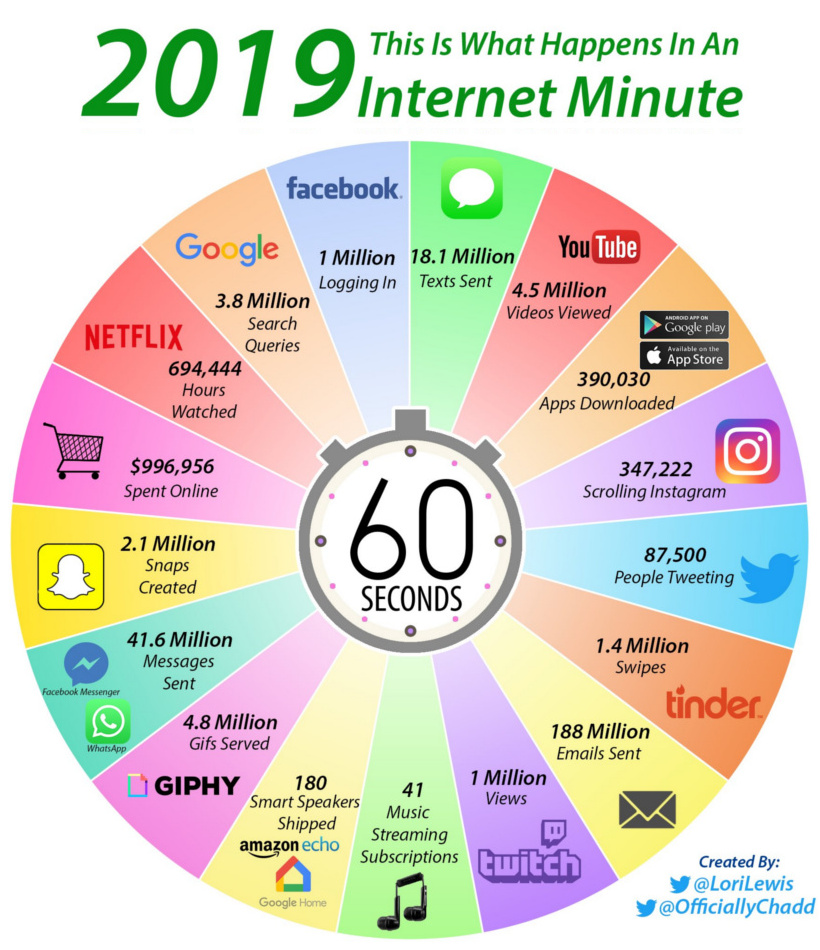
\includegraphics[width=0.5\textwidth]{images/internet-minute-2019.jpg}
    \caption{Ce qu'il se passe sur Internet en une minute en 2019 \citep{desjardins_what_2019}}
    \label{fig:internet_minute_2019}
\end{figure}

\paragraph{}
Avec une telle quantité de données, les exemples pour "apprendre à marcher" ne manquent pas. Bien évidemment, les machines apprennent différemment des humains. Il existe plusieurs types d'apprentissage, mais deux sont très répandus : l'apprentissage supervisé et l'apprentissage non supervisé.

\paragraph{L'apprentissage supervisé}
Ce type d'apprentissage correspond au fait de généraliser une règle à partir d'exemples annotés avec des labels\footnote{Un label correspond à la cible de la prédiction : par exemple pour prédire un email est un spam, le label sera le fait qu'un email est un spam ou non.}. Dans cette catégorie, il y a deux sous-groupes : la classification et la régression.

\paragraph{}
La classification cherche à prédire une classe, par exemple pour classer un email comme spam ou non, ou si un patient est atteint d'un cancer. En d'autres termes il s'agit de prédire une information non numérique. Logiquement, la régression correspond à une prédiction d'une valeur numérique comme le prix d'une maison ou la température moyenne de demain. Sur la figure \ref{fig:apprentissage_supervise}, il est possible de voir que pour la classification, il s'agit de séparer les classes pour prédire, alors que pour la régression, il est nécessaire d'avoir une fonction qui retourne un nombre.

\begin{figure}[hbt!]
    \centering
    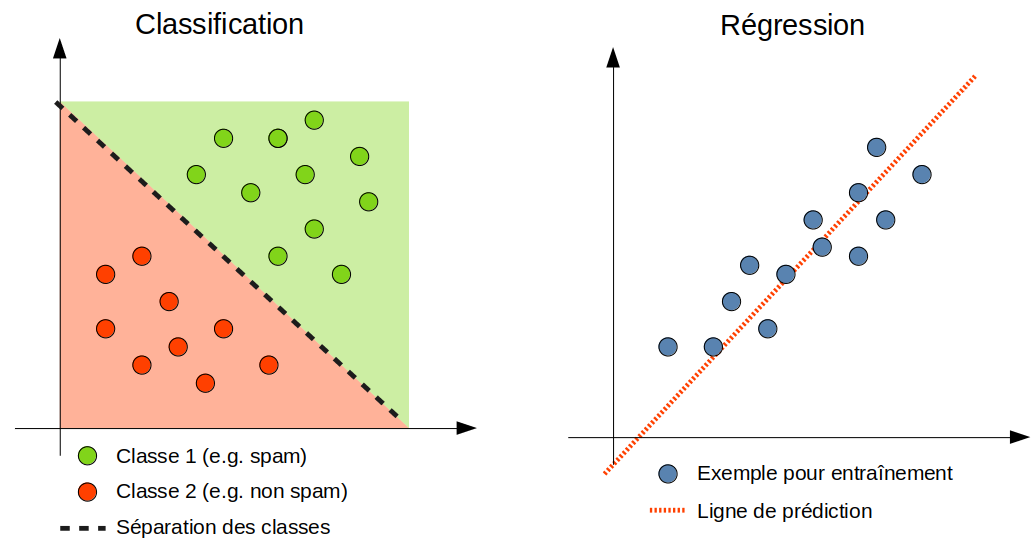
\includegraphics[width=\textwidth]{images/apprentissage_supervise.png}
    \caption{Représentation de l'apprentissage supervisé.}
    \label{fig:apprentissage_supervise}
\end{figure}

\paragraph{L'apprentissage non supervisé}
Cette catégorie d'apprentissage s'oppose au supervisé car les données ne sont pas annotées avec des labels. Les problématiques d'intelligence artificielle associées sont donc différentes. Généralement il s'agit de regrouper les données en différents groupes (Clustering) ou alors de détecter les éléments anormaux (détection d'anomalies), voir figue \ref{fig:apprentissage_non_supervise}.

\begin{figure}[hbt!]
    \centering
    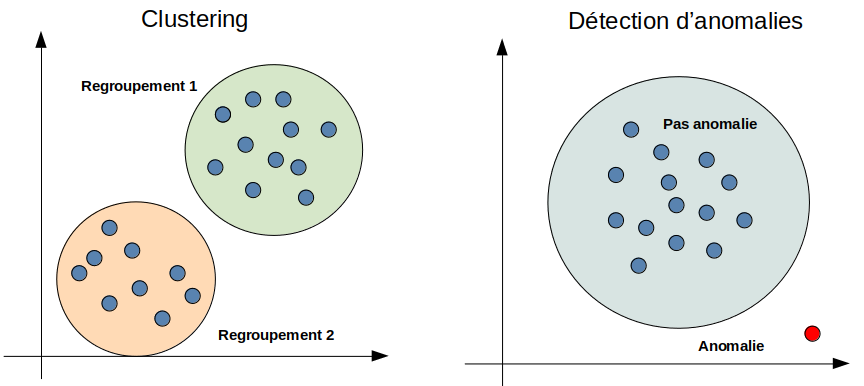
\includegraphics[width=\textwidth]{images/apprentissage_non_supervise.png}
    \caption{Représentation de l'apprentissage non supervisé.}
    \label{fig:apprentissage_non_supervise}
\end{figure}

\paragraph{}
Ces deux types d'apprentissage ont en commun leur processus de création. Cette logique est essentielle puisqu'elle permet de bien assimiler les mécanismes sous-jacents.

\subsubsection{La processus de fabrication}

Bien que chaque projet de Machine Learning soit différent sur le fond, la forme suit globalement la même logique. La première partie se concentre sur les données (collecte, exploration et préparation) pour ensuite se recentrer sur le modèle\footnote{Un modèle est un algorithme d’intelligence artificielle (modèle mathématique, statistique).} qui servira à résoudre la problématique choisie. Les grandes lignes qui vont être décrites en suivant se basent sur les articles de Matthew Mayo (KDnuggets)\footnote{https://www.kdnuggets.com/2018/12/machine-learning-project-checklist.html} et de Jeremy Jordan\footnote{https://www.jeremyjordan.me/ml-projects-guide/}.

\paragraph{Définition du problème}
L'objectif du projet est décidé dans cette section. Tout
d'abord une définition en terme métier est nécessaire, soit en langage naturel sans parler technique. Une fois que la problématique est définie une reflexion doit être entamer sur les composants technique du projet. Il s'agit de défnir les données souhaitées, comment les récupérer, quel type d'algorithme va être choisi (classifcation, régression, clustering, etc.), les décisions qui seront prises à partir des prédictions du modèle ou encore comment évaluer la performance du modèle. L'importance de cette étape est surtout sur la question de la faisabilité. Pour y répondre, il y a nécessité de déterminer le coût de l'acquisition des données, le coût de mauvaises prédictions, la quantité de travaux publiés sur un problème similaire et encore si l'environnement informatique ne contraindra pas le modèle \citep{jordan_organizing_2018}.

\paragraph{Collecte}
Cette étape consiste à faire le pont entre la définition des données en langage naturel avec leur localisation physiques (base de données, fichier de données, etc.). Il est important d'être sûr que cette acquisition de données respecte les réglementations qui les concerne (e.g. RGPD\footnote{Le Réglement Général sur la Protection des Données est une loi en vigueur depuis mai 2018 dans les pays de l'UE.}). Une fois les données récupérées, s'assurer qu'elles ont le bon type associé \citep{mayo_machine_2018}.

\paragraph{Analyse des données}
Cette étape est plus connu sous le nom d'analyse exploratoire des données (Exploratory Data Analysis, EDA en anglais). Son rôle est de comprendre ce qui compose les données, par exemple est-ce qu'il y a plus d'hommes que de femmes. La clé pour bien réussir cette section est la visualisation par des graphiques. Si l'analyse est bien faite, montrer les résultats à d'autres personnes ne connaissant pas le sujet et constater s'ils comprennent l'histoire racontée par ces données est un bon indicateur. De plus, c'est ici qu'il faut s'assurer que les données soient de qualité : qu'elles ne soient pas fausses (e.g. email mal renseigné).

\paragraph{Préparation}
Pour faire un plat en cuisine avoir les ingrédients et une recette correspond aux première étapes, mais il faut préparer les ingrédients en lisant la recette pour avoir le résultat souhaité. La préparation des données suit la même logique, l'analyse des données permet de savoir comment préparer les données (e.g. supprimer des informations inutiles). Cette étape est plus communément également appelée "Feature engineering" en anglais \citep{mayo_machine_2018}.

\paragraph{Création du modèle}
Les étapes précédentes sont cruciales pour permettre la qualité des données avant qu'elles soient digérées par le modèle, en général elles représentent 75\% du temps de travail d'un Data Scientist \citep{figure_eight_state_2019}. Les compétences requises pour réaliser la création du modèle sont orientées vers les mathématiques puisque un modèle est en général un algorithme paramétrable. Quand le modèle est sélectionné, s'en suit l'apprentissage en utilisant les données (C.F. section \ref{subsubsection:ia_auj}).

\paragraph{Validation du modèle}
Une fois entrainée, l'IA doit être testée et validée. Comme pour des étudiants français en terminale passant le baccalauréat, chacun a eu son apprentissage et en fonction de leur note finale, il sera déterminé s'ils ont eu ou non leur diplôme. Ici la note à attribuer correspond à une mesure définie, l'une des plus utilisée en classification est la justesse (accuracy en anglais) des prédictions, soit le pourcentage de prédictions justes (C.F. équation \ref{eq:accuracy}).

\begin{equation}\label{eq:accuracy}
    Justesse = \frac{\text{Nombre de prédictions correctes}}{\text{Nombre total de prédictions}}
\end{equation}

\paragraph{Déploiement}
Le déploiement du modèle fait appel à la casquette technique puisqu'il s'agit de rendre le modèle utilisable sur le long terme. Cette étape doit créer une "tuyauterie" reliant les données au modèle qui offre la prédition. 

\paragraph{Contrôle}
Enfin, une étape cruciale, mais qui est souvent oubliée, celle de la surveillance et du maintien de l'IA. Selon Figure Eight, seulement 37\% des développeurs maintiennent leurs modèles en permanence \citep{figure_eight_state_2019}. Si un problème est identifié, par exemple un nouveau comportement chez les clients que le modèle ne connait pas, il faut déterminer s'il faut juste ré-entrainer le modèle ou le cas échant, recommencer le processus de création de l'IA.  

\begin{center}
\begin{figure}[hbt!]
    \makebox[\textwidth]{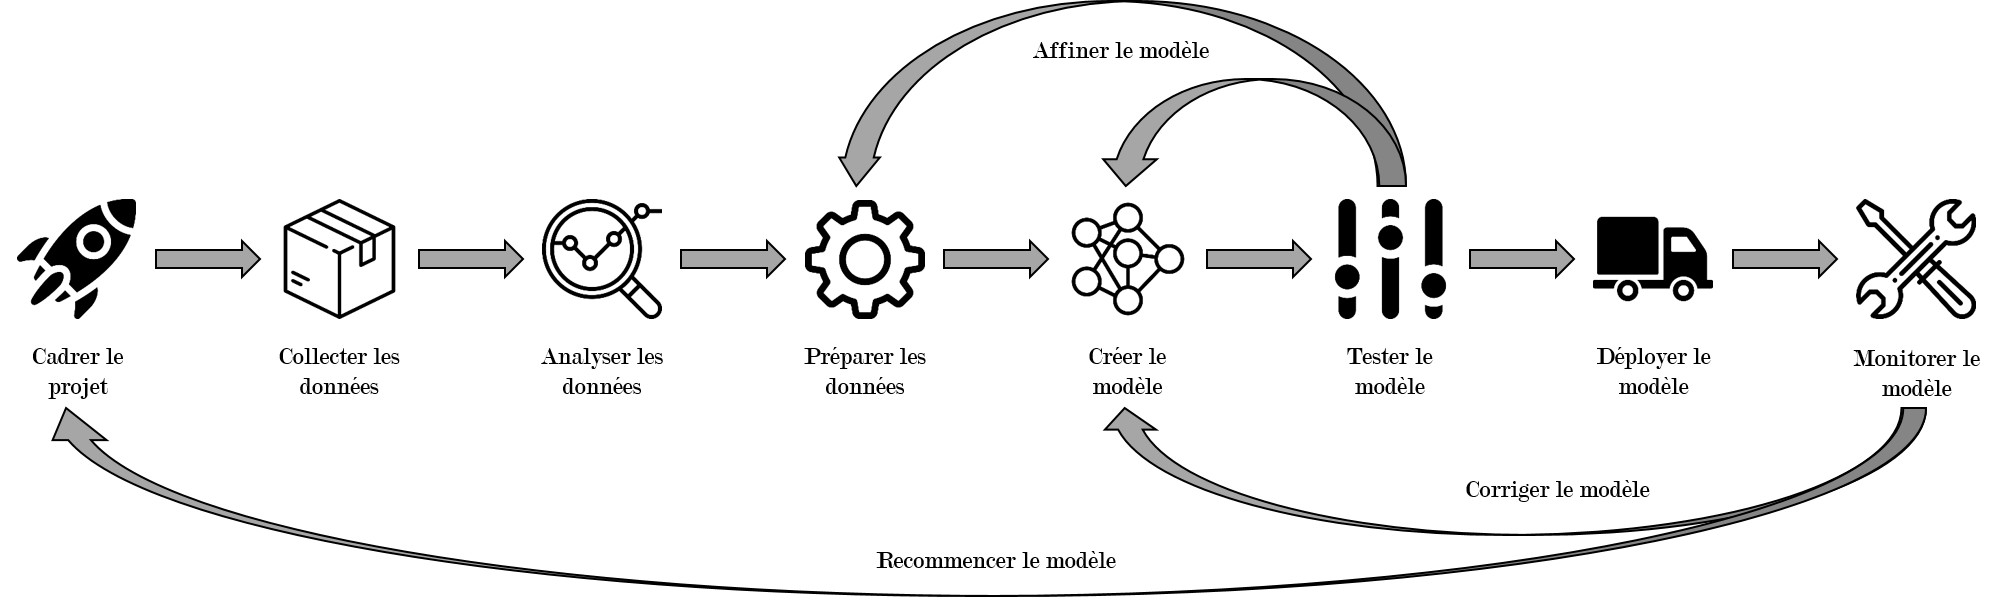
\includegraphics[width=0.9\paperwidth]{ressources/pipeline_ml_project.png}}
    \caption{Pipeline d'un projet de Machine Learning "classique". Crédit icônes \href{https://www.flaticon.com/}{Flaticon} : mynamepong, Freepik, Gregor Cresnar et Becris.}
\end{figure}
\end{center}

\paragraph{}
Le passé, le futur et le présent des algorithmes intelligents sont étroitement liés aux humains. Si savoir comment évolueront les IA dans un futur plus ou moins lointain, comprendre la morale et l'éthique de notre espèce peut apporter un élément de réponse.

% ------ ETHIQUE ------ %

\subsection{L’éthique, la science de la morale}
\label{subsec:ethique}

\paragraph{}
Le bien et le mal sont souvent deux notions assez abstraites, que chacun assimile telle une doctrine de conduite qui nous inspire. Comment sont-elles définies ? Une question sur laquelle la notion de morale est présente. Issu du latin "moralis" signifiant "relatif aux mœurs", ce mot s’inscrit au centre de la lutte entre le bien et le mal relatif à chaque individu pour créer des formes de normes morales en société. Cela affirme nos devoirs, droits ou encore interdits (au-delà même des lois).

\paragraph{}
Le code de conduite qui récite ce qui est de l’ordre du devoir pour femmes et hommes, aussi appelé éthique (synonyme de morale), est apparu d’un besoin de coopération à l’époque des chasseurs-cueilleurs. En effet, l’égoïsme favorise l’individu et non le groupe, or dans des temps où la survie passait par le social et le groupe, un comportement individualiste diminuait les chances de survie \citep{harari_sapiens:_2015}.

\paragraph{}
L'éthique, un terme assez générique donc, mais souvent porté dans l’illusion d’un absolu, plus précisément, la morale est parfois pensée comme une morale universelle. Or à la question : "Y a-t-il une morale universelle ?" (signifiant qui vaut en tout temps et en tous lieux), la réponse semble être négative.

\paragraph{}
L’ambiguïté de cette idée vient certainement de l’ethnocentrisme\footnote{Terme introduit par William Graham Summer, sociologue, signifiant l’évaluation d’autres civilisations d’après des critères qui sont en réalité les nôtres, mais dont il est pensé qu’ils sont universels} \citep{sumner_folkways_1906}, une généralisation abusive de nos critères moraux. La morale est le reflet d’un contexte social et temporel. Un exemple frappant est celui du vol. Perçu dans notre époque comme un acte voyou, du temps des Spartiates, le vol faisait partie de l’éducation des jeunes hommes dans le but de compléter leurs rations de nourriture \citep{ducat_du_2017}.

\paragraph{}
La notion d’universalité mise de côté, la question la plus adéquate sera de penser sur le plan de l’objectivité. C'est pourquoi, pour définir une morale, il faut revenir sur l'origine du bon, du méchant ou encore du mauvais caractérisant le bien et le mal. En d'autres termes, il faut regarder comment se compose une morale, en philosophie.

\subsubsection{L'origine du bon}
\label{subsec:ethique_origine_bon}

\paragraph{}
Le terme "bon", émet un jugement de valeur positif lorsqu’il est utilisé. Avec ce jugement, il est nécessaire d’y trouver son opposition, un linguiste de la Novlangue\footnote{La novlangue ou en anglais "Newspeak" est la langue officielle d’Ocania inventée par George Orwell dans son roman 1984, son principe est de diminuer le nombre de mots afin de diminuer le nombre de concepts servant à la réflexion. La négation des mots se formule en rajoutant le terme "in" en début de mot.} dirait "Inbon", mais cela n’est pas le mot recherché en français. Deux termes semblent être de bons candidats : mauvais et méchant. Alors, lequel serait le plus judicieux ?

\paragraph{}
L’origine de la morale, donc de l’opposition au "bon" a été analysé par Friedrich W. Nietzsche \citep{nietzsche_genealogie_1900} dans son livre "Généalogie de la morale". Ce texte cherche l’origine à la fois historique et psychologique. De nos jours, lorsqu’une action est dite bonne, il est souvent pensé qu’elle est altruiste soit bénéfique aux autres. Or dès le début du chapitre "Bien et mal", "Bon et mauvais", Nietzsche en parle pour renier cette origine du bénéfice global : "le jugement ‘‘bon’’ ne provient nullement de ceux qui bénéficient de cette ‘‘bonté’’ !". Il détaille par la suite que le fondement du bon a été créé par "les nobles, les puissants, les supérieurs en position et en pensée". Cette morale est l’expression de la puissance, de la force, elle célèbre soi-même. Ces "nobles", triomphants, posent ce qu’ils sont, ce qu’ils font comme valeurs "bonnes", c’est "la morale des maîtres".

\paragraph{}
L’opposition de bon, dans cette morale, est alors le mauvais : celui qui veut être bon, mais qui ne peut pas. Cette vision de l’éthique peut paraître perturbante, mais l’expression "réussir dans la vie" évoque cette célébration de soi, cette opposition entre ceux qui sont bons dans leur vie et ceux qui échouent, qui sont mauvais. Bien qu’elle ne soit plus une morale majoritaire, des personnes semblent en être adeptes.

\paragraph{}
Toujours dans le même chapitre de la "Généalogie de la morale", Nietzsche évoque à répétition, une haine qui se produit contre les "maîtres", ceux qui se qualifient de bons. Les humains, qui dans une logique de morale de maître, seraient alors mauvais, y voient quelque chose de méprisable dans cette réussite puisqu’ils ne peuvent l’atteindre. C’est à partir de cela, dans le ressentiment, qu’une morale a émergé et a dominé la morale du bon et du mauvais, "la morale des esclaves".

\paragraph{}
Elle se fonde sur la désapprobation des autres, de leurs actes, de leurs pensées, contre les méchants : ceux qui peuvent être bons, mais ne le veulent pas. En effet, le mauvais est devenu le bon et le bon est devenu le méchant.

\paragraph{}
Heureusement, il ne s’agit pas des seules morales sur Terre au XXIe siècle, elles ne semblent plus d’actualité. Cependant, leur existence est très importante sur le plan historique, de voir que les actions dites "bonnes" n’auront pas la même signification selon l’interlocuteur qui est en face. Mais alors, chacun possède-t-il une morale qui lui est propre ?

\subsubsection{Le jugement de chacun}
\label{subsec:ethique_jugement_chacun}

\paragraph{}
L’idée d’une morale personnelle, comme chaque individu possède des goûts, s’appelle le relativisme moral, soit une vision subjective de la morale. Cette doctrine prône le fait que les valeurs morales ne peuvent être évaluées objectivement. Cela signifie que tous jugements moraux sont uniquement issus de la culture à laquelle ils appartiennent. Ce mouvement s’oppose à ce qui est appelé le réalisme moral qui par opposition admet qu’il y a des valeurs morales objectives.

\paragraph{}
Dans cette pensée du réalisme, une branche morale est assez populaire, celle de la déontologie. Venant du grec "deon" signifiant devoir (la science du devoir), ce mouvement de pensée de la philosophie morale explique qu’il existe des devoirs moraux absolus soit sous la forme verbale "tu dois", et ce, sans rajouter une explication à ce devoir\footnote{Par exemple, "tu dois aider ton prochain", mais sans rajouter une justification.}. Ce principe fondamental, qui est appelé un impératif catégorique, est issu du philosophe Emmanuel Kant dans son ouvrage "Fondement sur la métaphysique des mœurs" \citep{kant_fondements_2007}.

\paragraph{}
Bien qu’il y ait des désaccords sur le fond entre déontologues, la forme en reste la même : celle d’un "tu dois" absolu. Il ne repose donc pas sur quelque chose de factuel et par conséquent, il peut être difficile de pouvoir arbitrer sur des actes immoraux.

\paragraph{}
Si le débat de l’arbitrage se déplace sur les faits dus à une action, aux conséquences engendrées, la morale qui s’appliquera sera le conséquentialisme. Elle se base sur les conséquences et sur le fait qu’elles seront négatives ou positives. Bien sûr, lorsque le terme "conséquence" est utilisé il s’agit des conséquences attendues et non réelles. La raison en est simple, il est souvent impossible de prévoir l’aboutissement d’une action bien après : si un enfant est sauvé de la noyade, comment prédire qu’il deviendrait un tueur en série trente ans plus tard.

\paragraph{}
Alors, comment juger moralement si une action est bonne ou mauvaise ? L’altruisme (une forme de conséquentialisme) y répond en établissant comme prémisse\footnote{Il s'agit d'une proposition avancée afin de supporter une conclusion, dans le cas de l'altruisme : optimiser le bonheur de tous.} de viser le bonheur de tous.

\paragraph{}
Une rivalité idéologique existe entre conséquentialisme et déontologie. En effet, pour les déontologues, l’idée est qu’un principe est bon donc qu’il est catégorique, pour un conséquentialiste, il y a des bonnes et des mauvaises situations et il faut faire le choix de la situation considérée comme bonne.

\paragraph{}
La forme pour savoir quelle est la bonne morale reste une matière à débattre forte intéressante, mais au travers de ces différentes visions de l’éthique, le fond semble à chaque fois rester cohérent et cela se voit bien aujourd’hui : un grand ensemble de lois sanctionne quand il s’agit d’un acte tel un meurtre ou un vol. Le contenu, qui semble se traduire au travers de certaines lois, porte également sur des débats d’idées, c’est pour cela qu’une vision conséquentialiste permet de raisonner de facto.

\paragraph{}
Tout ce raisonnement reste sur un plan philosophique. Il est important de savoir que chaque individu acquiert au cours de sa vie, une vision idéologique propre de la morale, son code d’éthique. C’est un processus qui commence dès la naissance avec notamment la théorie du développement moral \citep{kohlberg_moral_1977}, puisque notre appartenance à un groupe social défini déjà une partie de ce dont il adviendra de nos croyances, puis l’éducation rentre en jeu, l’entourage, etc.

\paragraph{}
Chaque humain peut être soumis à des biais\footnote{Un biais fait référence à une déviation de la réalité, un moyen de contourner} qui le feront agir pour une cause plutôt qu’une autre. Il est possible d’interpréter la morale d'un individu, mais concernant une machine intelligente, si la singularité est atteinte, le questionnement sera de savoir si la morale de l'algorithme correspond à celle de ses créateurs ou à une morale qui lui est propre.


% ------ IA et éthique ------ %

\subsection{La question de l'éthique pour les algorithmes intelligents}
\label{subsec:ia_ethique}

\paragraph{}
Dans les parties précédentes, il a été question du concept de l’intelligence artificielle et également de la notion de singularité, puis la réflexion s’est focalisée sur la question de l’éthique, science de la morale. Se questionner sur une morale au sein d’un algorithme intelligent peut avoir plusieurs aspects : l’éthique de la machine ou bien celle de la femme ou homme responsable de sa création, qu’il s’agisse de la vision éthique de l’humain ou de la société en charge.

\paragraph{}
Bien définir ce qu'est l'éthique pour une intelligence artificielle n'est pas chose facile, mais les codes moraux qui nous entourent ainsi que les lois permettent d'avoir une intuition (subjective) par rapport à cette problématique. Puisqu'il n'y a pas de morale universelle (C.F. section \ref{subsec:ethique}), il n'est pas possible d'avoir une définition de principes éthiques, objectivement applicables selon les différentes croyances morales.

\paragraph{}
L’éthique au sein du domaine des IA, de nos jours, correspond à plusieurs notions : transparence du modèle ou encore les biais présents dans l’algorithme. Cela étant d’actualité, un autre point essentiel est à évoquer, celui du futur. En effet, l’idée de la singularité pousse la réflexion à des considérations purement spéculatives sur les menaces existentielles de l’intelligence artificielle pour l’humanité \citep{villani_donner_2018}.

\subsubsection{Les biais et leurs méfaits}

\paragraph{}
Chez les humains, les biais, dans l’époque moderne, sont souvent sujets à manipulation sans même que nous nous en rendions compte. L’un des plus importants est le biais de confirmation, une tendance à valider des arguments allant dans une idéologie similaire ou de rejeter ceux qui sont en opposition sans même s’attarder sur le fond. Le terme garde tout son sens lorsqu’il s’agit des biais au sein des intelligences artificielles. Parmi les différents biais pour les machines, trois types attirent l’attention.

\paragraph{}
Le premier, se baptisant le biais de sélection, il s’agit du manque de diversité des données sur lesquelles l'IA apprend. En effet, une IA cherchant à reconnaître si une personne est chef d’entreprise, si son entraînement se base sur une majorité d’hommes par rapport aux femmes, alors l’algorithme reconnaîtra plus souvent des hommes en tant que chef d’entreprise. Il existe des méthodes afin de réduire ce biais : avoir un jeu de données représentatif et proportionnel, ou alors de mettre des poids\footnote{Un poids, dans un modèle, correspond à atténuer ou amplifier l'influence d'une variable.} en fonction des données \citep{tran_selection_2017}.

\paragraph{}
Le suivant se nomme biais d’interaction, son nom étant explicite, il correspond à un biais se formant au travers de l’interaction que les humains ont avec l’intelligence artificielle. Un exemple célèbre date de 2016, Microsoft sortit un compte Twitter sous l’appellation "@TayandYou" plus connu sous le nom TAY signifiant "Thinking about you"\footnote{Traduction : Pensant à toi.} . Son objectif était de converser avec les utilisateurs du réseau social Twitter. Très rapidement, elle s’est mise à publier des messages à caractères homophobes ou encore antisémites. Le problème venait alors des internautes dialoguant avec elle, lui écrivant des messages politiquement incorrects \citep{tual_peine_2016}.

\paragraph{}
Le dernier biais lui, correspond à un biais dû au passé : le biais implicite ou latent. L’analogie applicable à l’humain serait la notion de stéréotype, soit l’attribution inconsciente d’une qualité ou d’un défaut à une personne appartenant à une certaine catégorie sociale \citep{greenwald_implicit_1995}. Au travers de ce biais, il est possible de retrouver des stéréotypes du genre, de la couleur de peau ou encore de l’appartenance à une catégorie sociale (e.g. jeune, adulte). Ce biais a notamment été repéré, aux USA, sur l’algorithme appelé COMPAS\footnote{Correctionnal Offender Management Profiling for Alternative Sanctions : c’est une IA qui classifie le risque de récidivisme d’un criminel.}, pour lequel un criminel noir aurait deux fois plus de chance d’être considéré comme récidiviste par rapport à un blanc, alors qu’en réalité le taux de récidivisme entre noirs et blancs et approximativement le même \citep{larson_how_2016}.

\paragraph{}
Ces quelques biais, démontrent la complexité de créer un modèle "juste", si une intelligence artificielle serait plus transparente avec des informations sur son fonctionnement et expliquer le pourquoi d’une décision, cela permettrait déjà un premier pas vers une réduction des biais.

\subsubsection{Ouvrir la boîte noire}

\paragraph{}
Le terme "boîte noire" est très important, il ramène à un algorithme totalement opaque pour lequel tout ce qu’il est possible d’avoir est une sortie à partir de données fournies en entrée. Alors, la problématique de comprendre ce qu’il se passe à l’intérieur de ces machines est primordiale afin de pouvoir avoir confiance en elles.

\paragraph{}
Dans un premier temps, les concepteurs des algorithmes (souvent ayant des compétences en mathématiques et en informatique) les plus utilisés de nos jours, pourraient très bien comprendre le pourquoi du comment des IA. La réalité ne conte pas cette histoire, en effet, pour certains types de modèles mathématiques, il est impossible d’interpréter ce qu’il se passe dedans. L’interprétabilité se définit par la description des éléments internes d’un système d’une manière compréhensible pour l’homme \citep{gilpin_explaining_2018}.

\paragraph{}
La figure \ref{fig:interpretabilite_ia} illustre en abscisse l’interprétabilité d’un modèle et en ordonnée sa performance, la corrélation à noter est que, plus un algorithme est performant, moins il est interprétable. Ce graphique illustre bien une problématique éthique sur le plan de la transparence d’une IA.

\begin{figure}[hbt!]
    \centering
    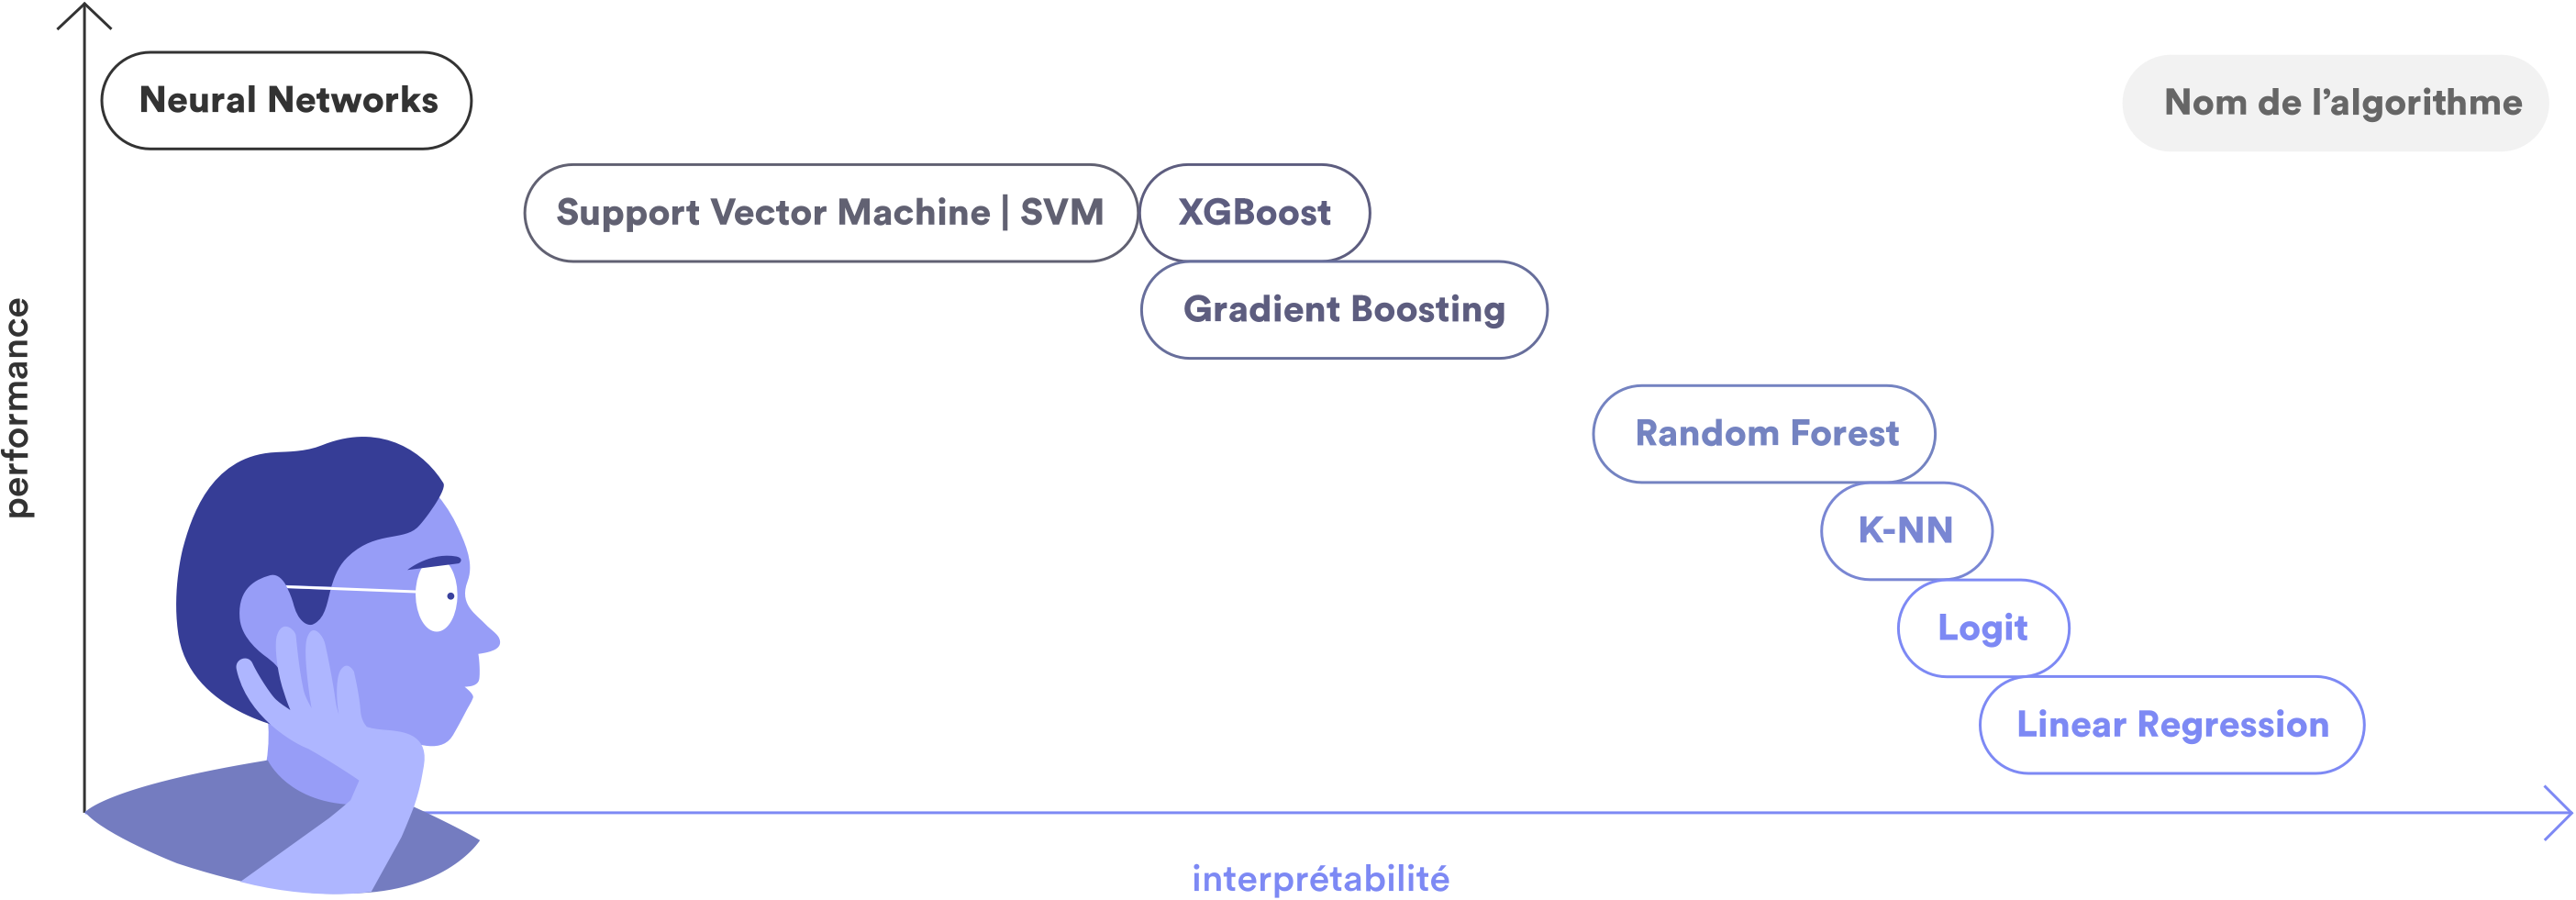
\includegraphics[width=\textwidth]{images/interpretabilite_ia.png}
    \caption{Interprétabilité d'un algorithme \citep{data_for_good_serment_2018}}
    \label{fig:interpretabilite_ia}
\end{figure}

\paragraph{}
Alors, la résignation d’avoir des algorithmes compréhensibles par l’humain est-elle nécessaire ? Non, rentre en jeu la notion d’explicabilité d’un modèle. Ce terme renvoie principalement à la question "Pourquoi ?", la capacité à répondre à ce questionnement lors d’une décision ou prédiction d’un modèle \citep{gilpin_explaining_2018}.

\paragraph{}
Concernant cette nouvelle problématique, l’explicabilité est plus facile à concevoir, pour reprendre la notion de boîte noire, il suffit de modifier les données en entrée pour voir comment cela influe sur le résultat obtenu par l’algorithme.

\paragraph{}
La transparence d’une intelligence artificielle passe également par la publication du code composant cette dernière publiquement, c’est-à-dire un code open-source\footnote{L’open source est une philosophie de développement désignant le fait d’ouvrir le code à tous, librement.}. Cela est bien problématique quand il s’agit d’algorithmes réalisés en entreprise et ne voulant pas publier leur réalisation au grand public.

\paragraph{}
Les explications à une non-<publication peuvent être diverses. Les plateformes comme Youtube ou Google ne publieront pas leur algorithme par nécessité d’éviter les abus afin de tirer profit d’une potentielle faille. OpenAI, eux bien qu’ils prônent cette idéologie de partager le code des IA afin de pouvoir mieux prévenir l’éthique des futures intelligences artificielles, ont décidé, de publier uniquement une partie de l’IA GPT-2 \citep{radford_language_2019}, IA capable d’écrire des textes catégorisables de "fake news"\footnote{Traduction : Informations fausses. Il s’agit de nouvelles pouvant sembler vraies dans la forme, mais fausses dans le fond.} et difficilement discernables par l’humain. La justification correspond au choix d’éprouver davantage le modèle et de laisser le temps de préparer des solutions aux problématiques amenées par ce modèle.

\paragraph{}
Cette difficulté, de rendre toutes les IA transparentes et compréhensibles par tous reflète bien le fossé séparant une éthique parfaite aujourd’hui et l’idéalisation qu’il est possible de faire, d’autant plus quand les algorithmes intelligents affectent notre quotidien. La responsabilité d’identifier les biais et comment rendre l’IA transparente revient dans un premier temps aux personnes s’occupant de la création des intelligences artificielles.

\subsubsection{Derrière chaque grande IA, des humains}

\paragraph{}
Ces dernières années, le quotidien d’une grande majorité de Français (ou autres habitants d’un pays catégorisé comme occidental) a énormément changé. En effet, suivant un rythme de croisière, les algorithmes dictant le style de vie du quotidien se sont retrouvés omniprésents : Facebook, Google, Netflix, Youtube et d’autres. Ces intelligences artificielles affectent-elles notre vision du monde, notre vie au quotidien ? Les data scientists\footnote{Développeur.euse en charge de créer le modèle qui composera l’intelligence artificielle.}, parents des IA peuvent bien changer notre quotidien au travers de leurs enfants.

\paragraph{}
Facebook, le réseau social ayant le plus d’utilisateurs dans le monde avec deux milliards 320 millions d’utilisateurs \citep{clement_global_2019}, a déjà eu l’occasion de prouver son influence sur l’humeur des utilisateurs. L’algorithme, qui choisit quelles publications un utilisateur pourra voir sur son fil d’actualité, possède une puissance d’impact sur nos émotions : si l’IA affiche une majorité de publications uniquement positives ou uniquement négatives sur une semaine, les publications, et donc l’humeur, des utilisateurs suivra l’état d’esprit auquel ils ont été exposés \citep{kramer_correction_2014}. Une telle constatation pose alors la question de l’influence que peut avoir l’idéologie des concepteurs de l’algorithme qu’ils en aient conscience ou non.

\paragraph{}
Sur Internet, il est possible de nos jours de trouver des réponses à nos questions sur des moteurs de recherche comme Google, leader de ce domaine. Il est surprenant de savoir que depuis 2017, plus de vidéos Youtube sont vues que de recherches Google sont effectuées \citep{desjardins_infographic:_2018}. La promotion de vidéos par l’algorithme de Youtube, fait rentrer ses utilisateurs dans des bulles correspondant à "leurs goûts". Au même détriment que Facebook, la vision du monde d’un internaute est alors biaisée par cette plateforme.

\paragraph{}
Cette source de média en ligne, étant alors une source irréfutable de distraction, connaissance ou encore de culture, est pour chaque utilisateur une urne remplie de vidéos catégorisées. Le risque dans un environnement de ce type est qu’il y ai une fixation sur une catégorie précise de vidéos (poussant alors le biais de confirmation s’il s’agit d’une idéologie). Mickaël Launay soutient, qu’en mathématiques, un tel milieu ségrègue les utilisateurs en deux ensembles : les conformistes et anti-conformistes \citep{launay_urnes_2012}. Les conformistes auront uniquement des vidéos qui leur correspondent, mais pour la seconde catégorie les vidéos seront d’un certain pourcentage correspondant à leur goût et le reste étant dans la catégorie conforme.

\paragraph{}
L’influence des intelligences artificielles sur nos humeurs et opinions dans notre utilisation d’internet quotidienne est irréfutable. Bien que l’objectif de ses algorithmes est de maintenir ses utilisateurs le plus longtemps sur la plateforme, ces IA peuvent, malgré elles, pousser une addiction idéologique chez les utilisateurs. Les data scientists possèdent-ils les appétences pour des réflexions aussi poussées que les impacts sociaux issus de leurs intelligences artificielles ?

\paragraph{}
Une majorité de data scientists sont issus de formation statistique, mathématiques ou encore informatique. Cela contraint déjà sur la notion de connaissance du domaine sur lequel une IA sera développée. La responsabilité de ceux qui produisent les algorithmes intelligents est de mentionner dans leurs discours les limites de leurs travaux, mais aussi de fournir un maximum d’informations aux personnes prenant les décisions et législateurs qui devront évaluer l’impact potentiel de ces apports sur la société \citep{cointe_ethical_2017}. Si cette responsabilité n’est pas respectée ou pire, que les limites sont omises volontairement afin de profiter à l’entreprise créatrice alors les répercussions peuvent être de l’ordre des biais impactant des femmes et hommes n’en ayant point conscience.

\paragraph{}
L’objectif d’une conscience de l’éthique pour que les intelligences artificielles soient plus transparentes et moins biaisées, qu’elles soient plus justes, est bien présent dans la communauté des chercheurs. Malheureusement la conscience de cette problématique n’est pas majoritaire et dans le but de sensibiliser sur ce sujet, l’association Data for Good a mis en place le "Serment d’Hippocrate pour Data Scientist" \citep{data_for_good_serment_2018} prenant en compte ces problématiques. Bien que cela ne soit encore qu’un engagement n’ayant pas de valeur juridique, peut-être cela évoluera dans les années qui suivent.

\paragraph{}
Les valeurs qui sont évoquées dans ce document peuvent se résumer au nombre de cinq. Dans un premier temps, l’intégrité scientifique et la rigueur, puis la transparence vis-à-vis de l’information compréhensible par le plus de parties prenantes possibles. L’équité suit, afin de veiller à une égalité et d’éviter la discrimination de groupes. L’avant-dernière concerne le respect de la vie privée des personnes qui peuvent être touchées par les travaux réalisés et enfin la responsabilité poussant à assumer tout manquement ou en cas de conflit d’intérêt.

\paragraph{}
Cette conscience ne doit pas se limiter qu’aux concepteurs des IA, il est nécessaire que cela soit multi-disciplinaire. L’émergence des intelligences artificielles et la possibilité du passage de la singularité fait apparaître la difficulté à aligner la morale de l’homme à celle de la machine : c’est le problème de l’alignement.

\subsubsection{Expliciter la morale des humains pour l’IA}

\paragraph{}
Le futur qui admet une intelligence artificielle ayant un intellect supérieur à l’homme plonge dans les débats éthiques et culturels, le problème de l’alignement oblige l'écriture noir sur blanc de "la morale" souhaitée pour une machine. Cette démarche est nécessaire, la morale qu’une machine aurait dans le futur est difficilement conceptualisable pour les humains.

\paragraph{}
Pour ce faire, il serait intéressant d’avoir une liste de règles bien définies comme les célèbres trois lois de la robotique d’Isaac Asimov. Bien qu'elles soient recentrées sur l’atteinte et l’obéissance à l’être humain, le raisonnement est à pousser au maximum.

\paragraph{}
Une expérience de pensée assez célèbre pour illustrer cette nécessité serait le cas d'une voiture autonome, dans un contexte où les freins ne fonctionneraient pas en face de piétons, qui la voiture devrait choisir de tuer. Le MIT a proposé une étude nommée "Moral Machine", offrant des choix en fonction de l’âge, du nombre, du sexe, de la classe sociale (un exemple sur la figure \ref{fig:moral_machine}). Les résultats montrent une divergence entre les cultures. En effet pour la question de l’âge, la jeunesse sera préférée pour des pays dit occidentaux à contrario des pays asiatiques favorisant les personnes âgées \citep{awad_moral_2018}.

\begin{figure}[hbt!]
    \centering
    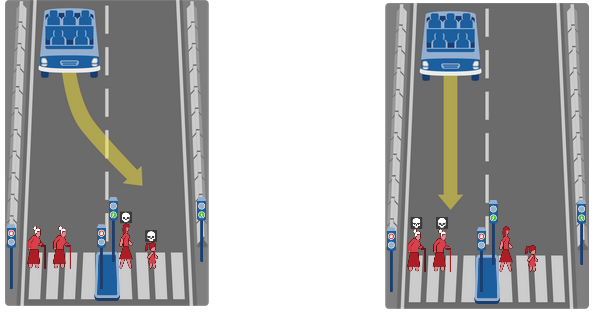
\includegraphics[width=\textwidth]{images/moral_machine.png}
    \caption{Expérience "Moral Machine" du MIT, ici le choix se pose entre deux femmes agées ou une petite fille accompagné d'une femme.}
    \label{fig:moral_machine}
\end{figure}

\paragraph{}
C’est déjà une étape importante puisque la réflexion émerge sur des questions qui sont d’actualité, e.g. la Californie autorisant les voitures autonomes à circuler sans conducteur \citep{shepardson_waymo_2018}, et permettent de commencer une réflexion plus profonde sur l’avenir de l’IA et d’une morale peut être relative à un pays. Tout ceci n’est que spéculation, les lois ne sont pas encore adaptées, les éthiques divergent énormément selon les pays.

\paragraph{}
Alors, si les lois sont plus difficilement malléables que les mœurs en rapport aux machines, des travaux ont été réalisés pour permettre dès l’apprentissage de l’algorithme intelligent de pouvoir aligner la morale humaine à celle de la machine.

\paragraph{}
Une solution pourrait être de découper la fabrication d’une IA en cinq parties : la collecte de données fiables, le modèle d’apprentissage basé sur la représentation du monde (issu des données collectées), la compréhension du modèle ainsi que le choix de la mesure de performance du modèle, définir les incentives\footnote{Il s’agit de source de motivation pour réaliser une action, e.g. une médaille lors d’une compétition sportive.} en jeux et enfin le renforcement de l’apprentissage dans le temps \citep{hoang_roadmap_2018}. Cette méthodologie s’axe sur tout le développement d’une IA, le point de départ pour parvenir à réaliser cela est de pouvoir conceptualiser les valeurs humaines.

\paragraph{}
La collecte des valeurs humaines dans le but de l’alignement passera par des questionnaires pour les humains, le problème étant que les réponses qui seront fournies posséderont des défauts : les biais, le manque de connaissances dans le domaine, les capacités cognitives limitées ou encore la culture dans laquelle évolue la femme ou l’homme. La nécessité d’inclure des sociologues avec chercheurs en IA est importante afin de répondre à la question de savoir si les humains donneront une bonne réponse à la question \citep{irving_ai_2019}.

\paragraph{}
La forme de l’apprentissage de la morale peut être appliquée sous diverses formes, par exemple l’une pourrait être par observation du comportement des autres et en ajustant la morale par l’observation des conséquences \citep{cointe_ethical_2017}. Une autre viserait plus l’apprentissage par le débat, poussant alors la justification des intelligences artificielles dans leurs recoins \citep{irving_ai_2019}.

\paragraph{}
La sensibilisation sur la problématique d’une morale pour les IA ainsi que le problème de l’alignement est primordiale. Il est important de travailler sur ces problèmes sur le plan technique en formant les actuels et futurs data scientists sur la question éthique et en rajoutant des sociologues pour aider sur les réponses aux questions de l’ordre moral, en d’autres termes, l’éducation et le social seront deux secteurs clés des avancées dans la transparence des algorithmes intelligents.

\paragraph{}
Tous ses problèmes que soulèvent les algorithmes intelligents, bien heureusement, suscitent un intérêt pour la communauté de chercheurs ainsi que pour les instances gouvernementales. Une volonté commune est née avec pour objectif de théoriser ce que peut être une intelligence artificielle éthique.

\subsubsection{Les cinq piliers hypothétiques d'une IA éthique}

\paragraph{}
La recherche sur l'IA éthique a fait couler de l'encre récemment, en effet les recommandations concernant cette dernière ne sont pas nouvelles, plus de 70 documents ont été publiés entre 2016 et 2019 par des entreprises, des gouvernements et des académies \citep{morley_what_2019}. Le but des auteurs de ces documents est qu'en définissant des principes théoriquement, de façon abstraite, ces principes permettront d'agir comme contraintes normatives \citep{turilli_ethical_2007} sur ce qui doit être fait et ce qui ne doit pas être empêché pour l'utilisation d'un algorithme. En d'autres termes, il s'agit de principes qui permettront de garantir une IA éthique.

\paragraph{}
En comparant les différents documents, cinq grands principes ressortent \cite{floridi_unified_2019}. Quatre d'entre eux sont ceux de la bioéthique\footnote{La bioéthique est l'étude des problèmes éthiques qui apparaissent avec les avancées en biologie et médecine \cite{beauchamp_principles_2009}.} : une IA doit être (a) bénéfique et respectueuse des humains et de l'environnement l'entourant (bienfaisance), (b) respectueuse des valeurs humaines (autonomie), (c) robuste et sécurisée (non-malfaisance) et (d) juste et équitable (justice). Le dernier est un nouveau, en effet le fait d'avoir une machine maîtresse de la décision change la donne. Une IA doit donc être (e) compréhensible par le plus grand nombre d'humains (explicabilité). Voir figure \ref{fig:principes_ia_ethique}.

\begin{figure}[hbt!]
    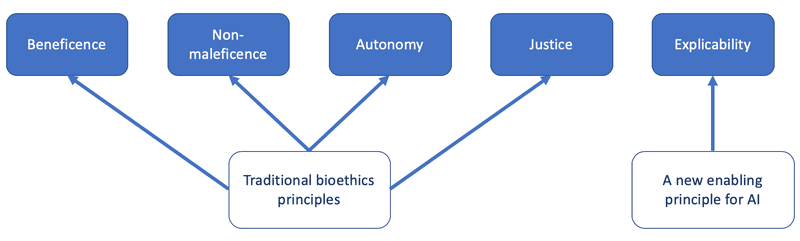
\includegraphics[width=\textwidth]{images/5_principles_ai_ethics.png}
    \caption{Les cinq principes d'une IA éthique \cite{floridi_unified_2019}.}
    \label{fig:principes_ia_ethique}
\end{figure}

\paragraph{}
Afin qu'une intelligence artificielle respecte ces principes, il est nécessaire d'implémenter des exigences pour chacun d'entre eux. La publication "Ethics guidelines for trustworthy AI"\footnote{Traduction : Directives éthiques pour une IA digne de confiance.} de la commission européenne, rassemblant des experts de l'IA, a pu définir des exigences pour clarifier la notion d'intelligence artificielle \cite{european_commission_ethics_2019}. Détaillons donc ce que sont ces cinq principes vitaux.

\paragraph{Bienfaisance}
Ce pilier correspond au bénéfice qu'un algorithme intelligent doit fournir aux humains. Dans un sens moral, il faut qu'elle soit bienveillante. En théorie, elle devrait promouvoir le bien-être, préserver la dignité et soutenir l'environnement \citep{floridi_unified_2019}.

\paragraph{}
Une IA ne devient pas bienveillante en un claquement de doigt, c'est donc dans ce pilier qu'il est nécessaire de poser la base morale de son algorithme. Plus communément appelé le problème de l'alignement des valeurs, il s'agit là de faire correspondre les valeurs humaines avec les valeurs de l'algorithme afin que les décisions prises soient en adéquation avec un code éthique \citep{russell_interview_2019}. 

\paragraph{}
Pour arriver à cette finalité, les différentes publications suggèrent les actions suivantes : 

\begin{itemize}
\item La participation des différents acteurs (commanditaires du projet, développeur et utilisateurs finaux), cela permettra de croiser les opinions et de s'assurer de la pertinence du sujet. 
\item Le respect des droits fondamentaux, garantissant les libertés primordiales pour tout être humain.
\item Durable et respectueuse de l'environnement : minimiser l'impact écologique qu'elle peut avoir, puisque le stockage de données ou l'entraînement d'un modèle de Machine Learning possède un coût environnemental.
\item La justification de l'IA : pourquoi elle devrait être créée, quels en seront les bénéfices pour les commanditaires.
\end{itemize}

\paragraph{Non-malfaisance}
Une IA ne doit pas porter atteinte à la vie privée des êtres humains et doit être également sécurisée. Il s'agit là d'avoir une vision responsable et de contrôler les risques sous-jacents. Le terme pour bien définir ce pilier serait la prévoyance.

\paragraph{}
Les doctrines "agir uniquement pour le bien" (bienfaisance) et "ne pas faire de mal" (non-malfaisance) semble être équivalentes, mais leurs objectifs sont en fait différents \citep{floridi_unified_2019}. Ne pas faire de mal correspond vraiment à anticiper le fait que des acteurs externes viennent perturber le bon fonctionnement de l'algorithme.

\paragraph{}
Afin de parvenir à cette prévoyance, il est nécessaire de suivre les directives suivantes :

\begin{itemize}
    \item La résilience par rapport aux attaques, s'assurer de la robustesse de l'algorithme quand les données en entrées sont perturbées. Par exemple, si quelqu'un ment sur son âge.
    \item Avoir un plan de secours : bien définir un processus pour s'assurer de la pérennité du modèle en cas de problème.
    \item La sécurité générale, vérifier que les logiciels et technologies utilisées soient à jour et sans failles de sécurité.
    \item Mesure de performance : s'assurer du bon fonctionnement du modèle avec une validation et un contrôle des performances.
    \item La qualité et l'intégrité des données : vérifier qu'il n'y a pas d'erreur dans la saisie, de la véracité de leur valeur.
    \item L'impact social : quels attributs sociaux sont pris en compte dans les données d'entraînement. Il faut également vérifier si une classe sociale (e.g. homme ou femme, marié ou célibataire) est favorisée ou non.     
\end{itemize}

\paragraph{Autonomie}
Contrôler les prédictions prises par un algorithme est essentiel, la notion d'autonomie s'axe principalement sur la construction d'une IA centrée autour de l'humain. Il s'agit là de l'habilité à décider, de pouvoir s'assurer que les machines ne soient pas complètement isolées.

\paragraph{}
La Déclaration de Montréal énonce la nécessité d'un équilibre entre les décisions prises par l'homme et celles prises par la machine, en déclarant que "le développement de l'IA devrait promouvoir l'autonomie de tous les êtres humains" \citep{universite_de_montreal_declaration_2017}. Le Groupe Européen sur l'éthique (EGE) soutient que les systèmes autonomes "ne doivent pas entraver la liberté des êtres humains de fixer leurs propres normes et standards" \citep{ege_ethics_2018}, tandis que le parlement de Grande-Bretagne adopte la position plus étroite selon laquelle "le pouvoir autonome de blesser, détruire ou tromper les êtres humains ne devrait jamais être dévolu à l'intelligence artificielle" \citep{uk_parliament_house_2017}.

\paragraph{}
La mise en application de cette notion passerait donc par les principes suivants :
\begin{itemize}
    \item La prise de décision passant par les humains, en fournissant des explications de la prédiction donnée par l'algorithme permettant alors une meilleure compréhension par la personne en charge.
    \item La surveillance dans le temps : s'assurer que la performance ne fléchisse pas avec le temps. 
\end{itemize}

\paragraph{Justice}
Promouvoir la prospérité, préserver la solidarité et éviter l'inégalité ou l'inéquité \citep{floridi_unified_2019}. L'un des problèmes d'un système autonome sur lequel l'humain n'a pas forcément un contrôle dans le processus algorithmique, c'est la capacité de savoir si l'algorithme est inéquitable, favorisant une classe sociale par rapport à une autre ou alors s'il reproduit des stéréotypes humains malgré lui, voire en créer de nouveaux.

\paragraph{}
Incorporer cette notion de justice, non dans le sens de l'instance avec un J majuscule, mais celui d'une IA équitable est d'autant plus essentiel que si cet aspect est oublié dans des secteurs fondamentaux comme la médecine ou la finance alors une nouvelle forme de discrimination pourrait apparaître, pouvant aller sur la vie même d'une personne.

\paragraph{}
Les principes à respecter seraient les suivants :
\begin{itemize}
    \item Éviter les biais inutiles, vérifier que l'algorithme ne perpétue pas des stéréotypes au cours du temps.
    \item Faire un design "universel" : si la restitution de l'information offerte par une IA est illisible cela peut créer une distance entre experts et non experts.
    \item Documenter les étapes de création de l'IA et assurer des contrôles réguliers.
    \item Définir les impacts négatifs potentiels, mais aussi leur déclaration et la minimisation en cas de problème.
    \item Anticiper les problèmes avec un mécanisme de correction.
\end{itemize}

\paragraph{Explicabilité}
Pour finir les cinq piliers, celui permettant d'assurer une communication entre l'humain et la machine. Une intelligence artificielle se doit d'être transparente et responsable. Pour le permettre, créer un moyen d'expliquer une décision ou prédiction, garanti une meilleure cohésion entre être humain et algorithme.

\paragraph{}
L'ajout du principe d'explicabilité, qui intègre à la fois le sens de l'intelligibilité (en réponse à la question "comment cela fonctionne-t-il ?") et le sens éthique de la responsabilité (en réponse à la question "qui est responsable de son fonctionnement ?"), est la pièce manquante essentielle du puzzle éthique pour l'intelligence artificielle \citep{floridi_unified_2019}.

\paragraph{}
Les concepts suivants sont des lignes de conduite pour mieux comprendre les IA :
\begin{itemize}
    \item La traçabilité permettant un suivi des prédictions dans le temps.
    \item La capacité d'expliquer avec un langage naturel comment la machine est parvenue à un résultat donné.
    \item Faire attention de ne pas avoir un algorithme non interprétable, soit compréhensible mathématiquement.
\end{itemize}

\paragraph{}
La force de ces cinq principes est dans le fait qu'ils touchent à une grande partie de ce qui compose les intelligences artificielles de nos jours. Derrière ces hypothèses décrite par la recherche, il y a un réel besoin puisque la réalité moderne démontre bien que ces algorithmes sont de plus en plus utilisés et un "contrôle éthique" n'est pas appliqué pour une vaste majorité de cas.

\subsection{Synthèse}

\paragraph{}
Pour rappel, la problématique de ce mémoire pose le cadre sur deux domaines : l’intelligence artificielle et l’éthique. Dans ce chapitre, dans un premier temps, l’histoire de l’intelligence a été évoquée avec notamment le test de Turing (voir section \ref{subsec:ia}). Celui-ci pouvant symboliser une première étape pour atteindre le passage de la singularité, qui, selon les experts du domaine aurait plus de cinquante pourcents de chances d’être atteinte d’ici cinquante ans (voir Figure \ref{fig:chrono_estim_ia}).

\paragraph{}
Dans un second temps, une introduction à la morale, avec entre autres son origine historiquo-philosophique vu par Nietzsche (voir section \ref{subsec:ethique_origine_bon}). Différentes morales ont été évoquées d’un point de vue philosophique démontrant une complexité déjà humaine à trouver une morale pouvant plaire au plus grand nombre (voir section \ref{subsec:ethique_jugement_chacun}).

\paragraph{}
C’est pour cela qu’en dernier lieu, la section \ref{subsec:ia_ethique} rentre dans les problèmes soulevés par l’intelligence artificielle sur le plan de l’éthique et présente un premier état de l’art sur les études existantes. Différents aspects ont été cités : les biais, la transparence des algorithmes, l’influence actuelle des IA avec les data scientists et enfin une vision qui pourrait permettre d’expliciter la morale des intelligences artificielles. De plus, cinq piliers hypothétiques ont été identifiés sur les recherches réalisées lors des années précédentes.

\paragraph{}
La problématique peut alors se découper sur trois points de l’éthique : moraliser les IA, la transparence et enfin les impacts sociaux que peuvent engendrer ces dernières.

\paragraph{}
Moraliser un algorithme revient à définir la vision de la morale que les créatrices et créateurs de ce dernier veulent lui attribuer, mais aussi à réfléchir aux biais que les données collectées peuvent posséder ou alors dans l’IA même.

\paragraph{}
La transparence s’axera sur l’interprétabilité du modèle, sa capacité à fournir des explications globales ou locales et enfin sur la possibilité ou non de rendre le code ouvert à tous.

\paragraph{}
Enfin, les impacts sociaux s’inscriront dans la démarche de poser les questions des conséquences que celui-ci peut avoir pour un groupe d’individus ou pour un cas particulier, qui est concerné et dans quels buts.

\paragraph{}
La vision qui ressort est celle d’une "méta-IA" soit d’une boîte à outil, d’un guide qui pourrait s’adapter aux différentes intelligences artificielles. Dans le chapitre suivant, je présente les différentes solutions déjà existantes pour permettre techniquement d'avoir une IA éthique puis je détaillerai la solution que j'ai créée, en expliquant sa nécessité.

% ====== SOLUTION ====== %

\newpage
\section{Solution proposée : une boîte à outil transparente}

% ------ Related works ------ %

\subsection{Outils existants}

\subsubsection{Cadrage}

\subsubsection{Analyse des données}

\subsubsection{Biais (données et modèle)}

\subsubsection{Explicabilité}

\subsubsection{Monitoring}

% ------ TransparentAI ------ %

\subsection{Une nouvelle solution : TransparentAI}

\subsubsection{Pourquoi cette solution ?}

\subsubsection{Description théorique et technique}

\subsubsection{Protocole de l'expérience}

\paragraph{Définir une / des hypothèse(s)}

FOCUS Expérience :

Définir ce qu'est une IA biaisée avec les formules mathématiques
Définir 2 / 3 idées d'IA (domaine bancaire) : Prérequis supervisé, prédiction concerne un individu et définir un objectif de performance correct avec expert métier
Choisir un type d'algo "simple" et un "complexe" qui sera appliqué pour chaque IA
Construire IA (sans TAI) avec obj la + perf possible
Construite IA (avec TAI) avec obj la - biaisée
Construite IA (avec TAI) avec obj meilleur compromis (définir compromis dans cadrage)
Comparer la performance et les biais pour chaque IA

\subsection{Synthèse}

% ====== RESULTATS ====== %

\newpage
\section{Résultats}

% ------ Déroulement ------ %

\subsection{Le déroulement}

% ------ Conclusions ------ %

\subsection{Les conclusions tirées}

% ------ Limites ------ %

\subsection{Les limites de l'expérience}

% ------ La suite ------ %

\subsection{La suite}

\subsection{Synthèse}

% ====== CONCLUSION ====== %

\newpage
\section{Conclusion}

\newpage
% \bibliographystyle{alpha}
\bibliographystyle{plainnat}
\bibliography{biblio}

\paragraph{1. Action humaine et contrôle humain}

\begin{center}
  \begin{tabular}{ |p{4cm}|p{6cm}|p{2cm}| } 
    \hline
    Aspect & Question & Tech ? \\
    \hline
    \hline
    Droits fondamentaux & Est-ce que l'utilisation de l'IA respecte les droits fondamentaux ? & Non \\
    \hline
    Action humaine & & Non \\
    \hline
    Contrôle humain & & Non \\ 
    \hline
    
  \end{tabular}
\end{center}

\paragraph{2. Robustesse technique et sécurité}

\begin{center}
  \begin{tabular}{ |p{4cm}|p{6cm}|p{2cm}| } 
    \hline
    Aspect & Question & Tech ? \\
    \hline
    \hline
    Résilience aux attaques et sécurité &  & Non \\
    \hline
    Solutions de secours et sécurité générale &  & Non \\
    \hline
    Précision &  & Non \\
    \hline
    Fiabilité et reproductibilité &  & Non \\
    \hline
    
  \end{tabular}
\end{center}

\paragraph{3. Respect de la vie privée et gouvernance des données}

\begin{center}
  \begin{tabular}{ |p{4cm}|p{6cm}|p{2cm}| } 
    \hline
    Aspect & Question & Tech ? \\
    \hline
    \hline
    Respect de la vie privée et protection des données &  & Non \\
    \hline
    Qualité et intégrité des données &  & Non \\
    \hline
    Accès aux données &  & Non \\
    \hline
    
  \end{tabular}
\end{center}

\paragraph{4. Transparence}

\begin{center}
  \begin{tabular}{ |p{4cm}|p{6cm}|p{2cm}| } 
    \hline
    Aspect & Question & Tech ? \\
    \hline
    \hline
    Traçabilité &  & Non \\
    \hline
    Explicabilité &  & Non \\
    \hline
    Communication &  & Non \\
    \hline
    
  \end{tabular}
\end{center}

\paragraph{5. Diversité, non-discrimination et équité}

\begin{center}
  \begin{tabular}{ |p{4cm}|p{6cm}|p{2cm}| } 
    \hline
    Aspect & Question & Tech ? \\
    \hline
    \hline
    Éviter les biais injustes &  & Non \\
    \hline
    Accessibilité et conception universelle &  & Non \\
    \hline
    Participation des parties prenantes & Est-ce qu'à minima, un.e des commanditaire, un.e développeur.se et un.e utilisateur.rice final.e ont pu participer au cadrage et à la validation du modèle ? & Non \\
    \hline
    
  \end{tabular}
\end{center}

\paragraph{6. Bien-être sociétal et environnemental}

\begin{center}
  \begin{tabular}{ |p{4cm}|p{6cm}|p{2cm}| } 
    \hline
    Aspect & Question & Tech ? \\
    \hline
    \hline
    IA durable et respectueuse de l’environnement &  & Non \\
    \hline
    Incidence sociale & Est-ce que le modèle peut avoir une incidence sociale sur un.e utilisateur.rice ? Par exemple, un risque de perte d'emploi ou un refus de crédit. & Non \\
    \hline
    Société et démocratie &  & Non \\
    \hline
    
  \end{tabular}
\end{center}

\paragraph{7. Responsabilité}

\begin{center}
  \begin{tabular}{ |p{4cm}|p{6cm}|p{2cm}| } 
    \hline
    Aspect & Question & Tech ? \\
    \hline
    \hline
    Auditabilité &  & Non \\
    \hline
    Minimisation et documentation des incidences négatives &  & Non \\
    \hline
    Documentation des arbitrages &  & Non \\
    \hline
    Voies de recours &  & Non \\
    \hline
    
  \end{tabular}
\end{center}

\end{document}
\end{document}